

\chapter{Lists  |  列表}

This chapter presents one of Python's most useful built-in types, lists.
You will also learn more about objects and what can happen when you have
more than one name for the same object.

本章介绍Python中最有用的内置类型之一:{\em 列表} (list)。 你还将进一步学习关于对象的知识以及同一个对象拥有多个名称时会发生什么。

\section{A list is a sequence  |  列表是一个序列}
\label{sequence}

Like a string, a {\bf list} is a sequence of values.  In a string, the
values are characters; in a list, they can be any type.  The values in
a list are called {\bf elements} or sometimes {\bf items}.

与字符串类似,{\em 列表} 是由多个值组成的序列。 在字符串中,每个值都是字符;
在列表中,值可以是任何数据类型。列表中的值称为 {\em 元素} (element) ,有时也被称为 {\em 项} (item)。

\index{list}  \index{type!list}
\index{element}  \index{sequence}
\index{item}

There are several ways to create a new list; the simplest is to
enclose the elements in square brackets (\verb"[" and \verb"]"):

创建新列表的方法有多种;最简单的方法是用方括号( \li{[} 和 \li{]} )将元素包括起来:

\begin{lstlisting}
[10, 20, 30, 40]
['crunchy frog', 'ram bladder', 'lark vomit']
\end{lstlisting}

%
The first example is a list of four integers.  The second is a list of
three strings.  The elements of a list don't have to be the same type.
The following list contains a string, a float, an integer, and
(lo!) another list:

第一个例子是包含 4 个整数的列表。第二个是一个包含 3 个字符串的列表。
一个列表中的元素不需要是相同的数据类型。下面的列表包含一个字符串、一个浮点数、一个整数和另一个列表:

\begin{lstlisting}
['spam', 2.0, 5, [10, 20]]
\end{lstlisting}

%
A list within another list is {\bf nested}.

一个列表在另一个列表中,称为 {\em 嵌套} (nested) 列表。
\index{nested list}  \index{list!nested}

A list that contains no elements is
called an empty list; you can create one with empty
brackets, \verb"[]".

一个不包含元素的列表被称为空列表;你可以用空的方括号 \li{[]} 创建一个空列表。

\index{empty list}  \index{list!empty}

As you might expect, you can assign list values to variables:

正如你想的那样,你可以将列表的值赋给变量:

\begin{lstlisting}
>>> cheeses = ['Cheddar', 'Edam', 'Gouda']
>>> numbers = [42, 123]
>>> empty = []
>>> print(cheeses, numbers, empty)
['Cheddar', 'Edam', 'Gouda'] [42, 123] []
\end{lstlisting}

%
\index{assignment}


\section{Lists are mutable  |  列表是可变的}
\label{mutable}
\index{list!element}  \index{access}
\index{index}  \index{bracket operator}
\index{operator!bracket}

The syntax for accessing the elements of a list is the same as for
accessing the characters of a string---the bracket operator.  The
expression inside the brackets specifies the index.  Remember that the
indices start at 0:

访问列表中元素的语法,与访问字符串中字符的语法相同,都是通过方括号运算符实现的。
括号中的表达式指定了元素的索引。记住,索引从0开始:

\begin{lstlisting}
>>> cheeses[0]
'Cheddar'
\end{lstlisting}

%
Unlike strings, lists are mutable.  When the bracket operator appears
on the left side of an assignment, it identifies the element of the
list that will be assigned.

和字符串不同的是,列表是可变的。当括号运算符出现在赋值语句的左边时,它就指向了列表中将被赋值的元素。

\index{mutability}

\begin{lstlisting}
>>> numbers = [42, 123]
>>> numbers[1] = 5
>>> numbers
[42, 5]
\end{lstlisting}

%
The one-eth element of {\tt numbers}, which
used to be 123, is now 5.

\li{numbers} 中索引为 1 的元素,原来是 123,现在变成了 5。
\index{index!starting at zero}  \index{zero, index starting at}

Figure~\ref{fig.liststate} shows the state diagram for {\tt
cheeses}, {\tt numbers} and {\tt empty}:
\index{state diagram}  \index{diagram!state}

图~\ref{fig.liststate} 展示了 \li{cheeses} 、 \li{nubmers} 和 \li{empty} 的状态图。

\begin{figure}
\centerline
{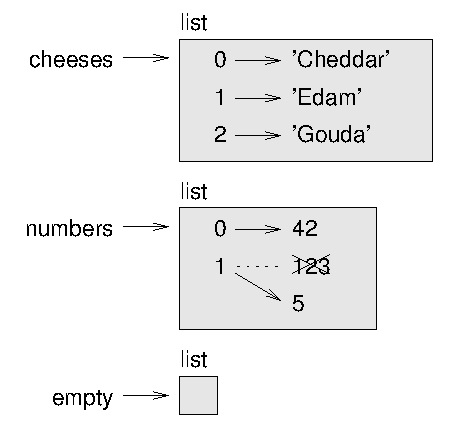
\includegraphics[scale=0.8]{../source/figs/liststate.pdf}}
% \caption{State diagram.}
\caption{状态图。}
\label{fig.liststate}
\end{figure}

Lists are represented by boxes with the word ``list'' outside
and the elements of the list inside.  {\tt cheeses} refers to
a list with three elements indexed 0, 1 and 2.
{\tt numbers} contains two elements; the diagram shows that the
value of the second element has been reassigned from 123 to 5.
{\tt empty} refers to a list with no elements.
\index{item assignment}  \index{assignment!item}
\index{reassignment}

列表用外部标有 ``list'' 的盒子表示,盒子内部是列表的元素。 \li{cheeses} 指向一个有3个元素的列表,3个元素的下标分别是0、1、2。 \li{numbers} 包含两个元素;
状态图显示第二个元素原来是123,被重新赋值为5。 \li{empty} 对应一个没有元素的列表。

List indices work the same way as string indices:

列表下标的工作原理和字符串下标相同:

\begin{itemize}

\item Any integer expression can be used as an index.

\item If you try to read or write an element that does not exist, you
get an {\tt IndexError}.
\index{exception!IndexError}  \index{IndexError}

\item If an index has a negative value, it counts backward from the
end of the list.

\end{itemize}

\begin{itemize}

\item 任何整数表达式都可以用作下标。

\item 如果你试图读或写一个不存在的元素,你将会得到一个 {\em 索引错误} (IndexError)。

\item 如果下标是负数,它将从列表的末端开始访问列表。

\end{itemize}
\index{list!index}  \index{list!membership}
\index{membership!list}  \index{in operator}
\index{operator!in}

The {\tt in} operator also works on lists.

\li{in} 运算符在列表中同样可以使用。

\begin{lstlisting}
>>> cheeses = ['Cheddar', 'Edam', 'Gouda']
>>> 'Edam' in cheeses
True
>>> 'Brie' in cheeses
False
\end{lstlisting}


\section{Traversing a list  |  列表遍历}
\index{list!traversal}  \index{traversal!list}
\index{for loop}  \index{loop!for}
\index{statement!for}

The most common way to traverse the elements of a list is
with a {\tt for} loop.  The syntax is the same as for strings:

最常用的遍历列表的方式是使用for循环。语法和字符串遍历类似:

\begin{lstlisting}
for cheese in cheeses:
    print(cheese)
\end{lstlisting}

%
This works well if you only need to read the elements of the
list.  But if you want to write or update the elements, you
need the indices.  A common way to do that is to combine
the built-in functions {\tt range} and {\tt len}:

如果你只需要读取列表中的元素,这种方法已经足够。 然而,如果你想要写入或者更新列表中的元素,你需要通过下标访问。一种常用的方法是结合内置函数 \li{range} 和 \li{len} :
\index{looping!with indices}  \index{index!looping with}



\begin{lstlisting}
for i in range(len(numbers)):
    numbers[i] = numbers[i] * 2
\end{lstlisting}

%
This loop traverses the list and updates each element.  {\tt len}
returns the number of elements in the list.  {\tt range} returns
a list of indices from 0 to $n-1$, where $n$ is the length of
the list.  Each time through the loop {\tt i} gets the index
of the next element.  The assignment statement in the body uses
{\tt i} to read the old value of the element and to assign the
new value.

这个循环将遍历列表并更新每个元素。 \li{len} 返回列表中的元素个数。 \li{range} 返回一个包含从 0 到 $n-1$ 下标的列表,其中 $n$ 是列表的长度。
每次循环中,\li{i} 得到下一个元素的下标。循环主体中的赋值语句使用 \li{i} 读取该元素的旧值,并赋予其一个新值。
\index{item update}  \index{update!item}

A {\tt for} loop over an empty list never runs the body:

对一个空列表执行 \li{for} 循环时,将不会执行循环的主体:

\begin{lstlisting}
for x in []:
    print('This never happens.')
\end{lstlisting}

%
Although a list can contain another list, the nested
list still counts as a single element.  The length of this list is
four:

尽管一个列表可以包含另一个列表,嵌套的列表本身还是被看作一个单个元素。
下面这个列表的长度是4:
\index{nested list}  \index{list!nested}

\begin{lstlisting}
['spam', 1, ['Brie', 'Roquefort', 'Pol le Veq'], [1, 2, 3]]
\end{lstlisting}


\section{List operations  |  列表操作}
\index{list!operation}

The {\tt +} operator concatenates lists:

{\em 加号运算符}\li{+} 拼接多个列表:

\index{concatenation!list}  \index{list!concatenation}

\begin{lstlisting}
>>> a = [1, 2, 3]
>>> b = [4, 5, 6]
>>> c = a + b
>>> c
[1, 2, 3, 4, 5, 6]
\end{lstlisting}

%
The {\tt *} operator repeats a list a given number of times:

{\em 乘号运算符} \li{*} 以给定次数的重复一个列表:
\index{repetition!list}  \index{list!repetition}

\begin{lstlisting}
>>> [0] * 4
[0, 0, 0, 0]
>>> [1, 2, 3] * 3
[1, 2, 3, 1, 2, 3, 1, 2, 3]
\end{lstlisting}

%
The first example repeats {\tt [0]} four times.  The second example
repeats the list {\tt [1, 2, 3]} three times.

第一个例子重复 4 次。 第二个例子重复了那个列表 3 次。

\section{List slices  |  列表切片}
\index{slice operator}  \index{operator!slice}  \index{index!slice}
\index{list!slice}  \index{slice!list}

The slice operator also works on lists:

{\em 切片} (slice) 运算符同样适用于列表:


\begin{lstlisting}
>>> t = ['a', 'b', 'c', 'd', 'e', 'f']
>>> t[1:3]
['b', 'c']
>>> t[:4]
['a', 'b', 'c', 'd']
>>> t[3:]
['d', 'e', 'f']
\end{lstlisting}
%
If you omit the first index, the slice starts at the beginning.
If you omit the second, the slice goes to the end.  So if you
omit both, the slice is a copy of the whole list.

如果你省略第一个索引,切片将从列表头开始。 如果你省略第二个索引,切片将会到列表尾结束。
所以如果你两者都省略,切片就是整个列表的一个拷贝。
\index{list!copy}  \index{slice!copy}
\index{copy!slice}

\begin{lstlisting}
>>> t[:]
['a', 'b', 'c', 'd', 'e', 'f']
\end{lstlisting}

%
Since lists are mutable, it is often useful to make a copy
before performing operations that modify lists.

由于列表是可变的,通常在修改列表之前,对列表进行拷贝是很有用的。
\index{mutability}

A slice operator on the left side of an assignment
can update multiple elements:

切片运算符放在赋值语句的左边时,可以一次更新多个元素:
\index{slice!update}  \index{update!slice}

\begin{lstlisting}
>>> t = ['a', 'b', 'c', 'd', 'e', 'f']
>>> t[1:3] = ['x', 'y']
>>> t
['a', 'x', 'y', 'd', 'e', 'f']
\end{lstlisting}

%

% You can add elements to a list by squeezing them into an empty
% slice:

% % \begin{lstlisting}
% >>> t = ['a', 'd', 'e', 'f']
% >>> t[1:1] = ['b', 'c']
% >>> print t
% ['a', 'b', 'c', 'd', 'e', 'f']
% \end{lstlisting}
% \afterverb
%
% And you can remove elements from a list by assigning the empty list to
% them:

% % \begin{lstlisting}
% >>> t = ['a', 'b', 'c', 'd', 'e', 'f']
% >>> t[1:3] = []
% >>> print t
% ['a', 'd', 'e', 'f']
% \end{lstlisting}
% \afterverb
%
% But both of those operations can be expressed more clearly
% with list methods.


\section{List methods  |  列表方法}
\index{list!method}
\index{method, list}

Python provides methods that operate on lists.  For example,
{\tt append} adds a new element to the end of a list:

Python为列表提供了一些方法. 例如, \li{append} 添加一个新元素到列表的末端:

\index{append method}  \index{method!append}

\begin{lstlisting}
>>> t = ['a', 'b', 'c']
>>> t.append('d')
>>> t
['a', 'b', 'c', 'd']
\end{lstlisting}
%
{\tt extend} takes a list as an argument and appends all of
the elements:

\li{extend} 将接受一个列表作为参数,并将其其中的所有元素添加至目标列表中:
\index{extend method}  \index{method!extend}

\begin{lstlisting}
>>> t1 = ['a', 'b', 'c']
>>> t2 = ['d', 'e']
>>> t1.extend(t2)
>>> t1
['a', 'b', 'c', 'd', 'e']
\end{lstlisting}

%
This example leaves {\tt t2} unmodified.

这个例子中 \li{t2} 没有改动。

{\tt sort} arranges the elements of the list from low to high:

\li{sort} 将列表中的元素从小到大进行排序:
\index{sort method}  \index{method!sort}

\begin{lstlisting}
>>> t = ['d', 'c', 'e', 'b', 'a']
>>> t.sort()
>>> t
['a', 'b', 'c', 'd', 'e']
\end{lstlisting}

%
Most list methods are void; they modify the list and return {\tt None}.
If you accidentally write {\tt t = t.sort()}, you will be disappointed
with the result.

大部分的列表方法都是无返回值的;它们对列表进行修改,然后返回None。
如果你意外的写了 \li{t.sort()}, 你将会对结果感到失望的。
\index{void method}  \index{method!void}
\index{None special value}  \index{special value!None}


\section{Map, filter and reduce  |  映射、筛选和归并}
\label{filter}

To add up all the numbers in a list, you can use a loop like this:

你可以这样使用循环,对列表中所有元素求和:

% see add.py

\begin{lstlisting}
def add_all(t):
    total = 0
    for x in t:
        total += x
    return total
\end{lstlisting}
%
{\tt total} is initialized to 0.  Each time through the loop,
{\tt x} gets one element from the list.  The {\tt +=} operator
provides a short way to update a variable.  This {\bf augmented assignment statement},

\li{total} 被初始化为 0。 每次循环时, \li{x} 从列表中获取一个元素。
运算符 \li{+=} 提供了一个快捷的更新变量的方法。 这个 {\em 增量赋值语句} (augmented assignment statement) 。

\index{update operator}  \index{operator!update}
\index{assignment!augmented}  \index{augmented assignment}

\begin{lstlisting}
    total += x
\end{lstlisting}

%
is equivalent to

等价于

\begin{lstlisting}
    total = total + x
\end{lstlisting}
%
As the loop runs, {\tt total} accumulates the sum of the
elements; a variable used this way is sometimes called an
{\bf accumulator}.

当循环执行时,\li{total} 将累计元素的和;一个这样的变量有时被称为 {\em 累加器} (accumulator) 。

\index{accumulator!sum}

Adding up the elements of a list is such a common operation
that Python provides it as a built-in function, {\tt sum}:

把一个列表中的元素加起来是一个很常用的操作,
所以Python将其设置为一个内建内置函数 \li{sum} :

\begin{lstlisting}
>>> t = [1, 2, 3]
>>> sum(t)
6
\end{lstlisting}
%
An operation like this that combines a sequence of elements into
a single value is sometimes called {\bf reduce}.

一个像这样的将一系列的元素合并成一个单一值的操作有时称为 {\em 归并} (reduce) 。

\index{reduce pattern}  \index{pattern!reduce}
\index{traversal}

Sometimes you want to traverse one list while building
another.  For example, the following function takes a list of strings
and returns a new list that contains capitalized strings:

有时,你在构建一个列表时还需要遍历另一个列表。  例如,下面的函数接受一个字符串列表

\begin{lstlisting}
def capitalize_all(t):
    res = []
    for s in t:
        res.append(s.capitalize())
    return res
\end{lstlisting}

%
{\tt res} is initialized with an empty list; each time through
the loop, we append the next element.  So {\tt res} is another
kind of accumulator.

\li{res} 被初始化为一个空列表;每次循环时,我们添加下一个元素。
所以 \li{res} 是另一种形式的累加器。

\index{accumulator!list}

An operation like \verb"capitalize_all" is sometimes called a {\bf
map} because it ``maps'' a function (in this case the method {\tt
capitalize}) onto each of the elements in a sequence.

类似 \li{capitalize_all} 这样的操作有时被称为 {\em 映射} (map) ,因为它 ``映射''一个函数(在本例中是方法 \li{capitalize} )到序列中的每个元素上。

\index{map pattern}  \index{pattern!map}
\index{filter pattern}  \index{pattern!filter}

Another common operation is to select some of the elements from
a list and return a sublist.  For example, the following
function takes a list of strings and returns a list that contains
only the uppercase strings:

另一个常见的操作是从列表中选择一些元素,并返回一个子列表。例如,下面的函数读取一个字符串列表,并返回一个仅包含大写字符串的列表:

\begin{lstlisting}
def only_upper(t):
    res = []
    for s in t:
        if s.isupper():
            res.append(s)
    return res
\end{lstlisting}

%
{\tt isupper} is a string method that returns {\tt True} if
the string contains only upper case letters.

\li{isupper} 是一个字符串方法,如果字符串仅含有大写字母,则返回 \li{True}。

An operation like \verb"only_upper" is called a {\bf filter} because
it selects some of the elements and filters out the others.

类似 \li{only_upper} 这样的操作被称为 {\em 筛选} (filter) ,因为它选中某些元素,然后剔除剩余的元素。

Most common list operations can be expressed as a combination
of map, filter and reduce.

大部分常用列表操作可以用映射、筛选和归并这个组合表示。


\section{Deleting elements  |  删除元素}
\index{element deletion}  \index{deletion, element of list}

There are several ways to delete elements from a list.  If you
know the index of the element you want, you can use
{\tt pop}:

有多种方法可以从列表中删除一个元素。如果你知道元素的下标,你可以使用 \li{pop} :

\index{pop method}  \index{method!pop}

\begin{lstlisting}
>>> t = ['a', 'b', 'c']
>>> x = t.pop(1)
>>> t
['a', 'c']
>>> x
'b'
\end{lstlisting}

%
{\tt pop} modifies the list and returns the element that was removed.
If you don't provide an index, it deletes and returns the
last element.

\li{pop} 修改列表,并返回被移除的元素。 如果你不提供下标,它将移除并返回最后一个元素。

If you don't need the removed value, you can use the {\tt del}
operator:

如果你不需要被移除的元素,可以使用 \li{del} 运算符:

\index{del operator}  \index{operator!del}

\begin{lstlisting}
>>> t = ['a', 'b', 'c']
>>> del t[1]
>>> t
['a', 'c']
\end{lstlisting}

%
If you know the element you want to remove (but not the index), you
can use {\tt remove}:

如果你知道要删除的值(但是不知道其下标),你可以使用 \li{remove} :

\index{remove method}  \index{method!remove}

\begin{lstlisting}
>>> t = ['a', 'b', 'c']
>>> t.remove('b')
>>> t
['a', 'c']
\end{lstlisting}
%
The return value from {\tt remove} is {\tt None}.

\li{remove} 的返回值是 \li{None}。

\index{None special value}  \index{special value!None}

To remove more than one element, you can use {\tt del} with
a slice index:

要移除多个元素,你可以结合切片索引使用 \li{del} :

\begin{lstlisting}
>>> t = ['a', 'b', 'c', 'd', 'e', 'f']
>>> del t[1:5]
>>> t
['a', 'f']
\end{lstlisting}

%
As usual, the slice selects all the elements up to but not
including the second index.


同样的,切片选择到第二个下标(不包含第二个下标)处的所有元素。


\section{Lists and strings  |  列表和字符串}
\index{list}  \index{string}
\index{sequence}

A string is a sequence of characters and a list is a sequence
of values, but a list of characters is not the same as a
string.  To convert from a string to a list of characters,
you can use {\tt list}:

一个字符串是多个字符组成的序列,一个列表是多个值组成的序列。 但是一个由字符组成的列表不同于字符串。可以使用 \li{list} 将一个字符串转换为字符的列表:

\index{list!function}  \index{function!list}

\begin{lstlisting}
>>> s = 'spam'
>>> t = list(s)
>>> t
['s', 'p', 'a', 'm']
\end{lstlisting}

%
Because {\tt list} is the name of a built-in function, you should
avoid using it as a variable name.  I also avoid {\tt l} because
it looks too much like {\tt 1}.  So that's why I use {\tt t}.

由于 \li{list} 是内置函数的名称,你应避免将它用作变量名。我同样避免使用 \li{l} ,因为它看起来很像 \li{1}。 这就是为什么我用了 \li{t} 。

The {\tt list} function breaks a string into individual letters.  If
you want to break a string into words, you can use the {\tt split}
method:

\li{list} 函数将字符串分割成单独的字符。 如果你想将一个字符串分割成一些单词, 你可以使用 \li{split} 方法:

\index{split method}  \index{method!split}

\begin{lstlisting}
>>> s = 'pining for the fjords'
>>> t = s.split()
>>> t
['pining', 'for', 'the', 'fjords']
\end{lstlisting}

%
An optional argument called a {\bf delimiter} specifies which
characters to use as word boundaries.
The following example
uses a hyphen as a delimiter:

可以提高一个叫做 {\em 分隔符} (delimiter) 的可选参数,指定什么字符作为单词之间的分界线。 下面的例子使用连字符作为分隔符:

\index{optional argument}  \index{argument!optional}
\index{delimiter}

\begin{lstlisting}
>>> s = 'spam-spam-spam'
>>> delimiter = '-'
>>> t = s.split(delimiter)
>>> t
['spam', 'spam', 'spam']
\end{lstlisting}

%
{\tt join} is the inverse of {\tt split}.  It
takes a list of strings and
concatenates the elements.  {\tt join} is a string method,
so you have to invoke it on the delimiter and pass the
list as a parameter:

\li{join} 的功能和 \li{split} 相反。 它将一个字符串列表的元素拼接起来。 \li{join} 是一个字符串方法,所以你需要在一个分隔符上调用它,并传入一个列表作为参数:

\index{join method}  \index{method!join}
\index{concatenation}

\begin{lstlisting}
>>> t = ['pining', 'for', 'the', 'fjords']
>>> delimiter = ' '
>>> s = delimiter.join(t)
>>> s
'pining for the fjords'
\end{lstlisting}

%
In this case the delimiter is a space character, so
{\tt join} puts a space between words.  To concatenate
strings without spaces, you can use the empty string,
\verb"''", as a delimiter.

在这个例子中,分隔符是一个空格,所以 \li{join} 在单词之间添加一个空格。如果不使用空格拼接字符串,你可以使用空字符串 \li{''} 作为分隔符。

\index{empty string}  \index{string!empty}


\section{Objects and values  |  对象和值}
\label{equivalence}
\index{object}  \index{value}

If we run these assignment statements:

如果我们执行下面的赋值语句:

\begin{lstlisting}
a = 'banana'
b = 'banana'
\end{lstlisting}

%
We know that {\tt a} and {\tt b} both refer to a
string, but we don't
know whether they refer to the {\em same} string.
There are two possible states, shown in Figure~\ref{fig.list1}.

我们知道 \li{a} 和 \li{b} 都指向一个字符串, 但是我们不知道是否他们指向 {\bf 同一个} 字符串。 这里有两种可能的状态,如 图~\ref{fig.list1} 所示。

\index{aliasing}

\begin{figure}
\centerline
{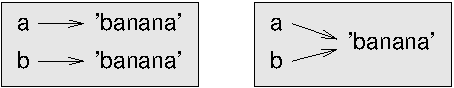
\includegraphics[scale=0.8]{../source/figs/list1.pdf}}
\caption{State diagram.}
\label{fig.list1}
\end{figure}

In one case, {\tt a} and {\tt b} refer to two different objects that
have the same value.  In the second case, they refer to the same
object.

一种情况是,\li{a} 和 \li{b} 指向两个有相同值的不同对象。
第二种情况是,它们指向同一个对象。

\index{is operator}  \index{operator!is}

To check whether two variables refer to the same object, you can
use the {\tt is} operator.

为了查看两个变量是否指向同一个对象,你可以使用 \li{is} 运算符。

\begin{lstlisting}
>>> a = 'banana'
>>> b = 'banana'
>>> a is b
True
\end{lstlisting}

%
In this example, Python only created one string object, and both {\tt
  a} and {\tt b} refer to it.  But when you create two lists, you get
two objects:

在这个例子中,Python仅生成了一个字符串对象,\li{a} 和 \li{b} 都指向它。 但是当你创建两个列表时,你得到的是两个对象:

\begin{lstlisting}
>>> a = [1, 2, 3]
>>> b = [1, 2, 3]
>>> a is b
False
\end{lstlisting}

%
So the state diagram looks like Figure~\ref{fig.list2}.

所以状态图如图~\ref{fig.list2}所示。

\index{state diagram}  \index{diagram!state}

\begin{figure}
\centerline
{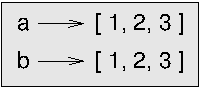
\includegraphics[scale=0.8]{../source/figs/list2.pdf}}
\caption{State diagram.}
\label{fig.list2}
\end{figure}

In this case we would say that the two lists are {\bf equivalent},
because they have the same elements, but not {\bf identical}, because
they are not the same object.  If two objects are identical, they are
also equivalent, but if they are equivalent, they are not necessarily
identical.

在这个例子中,我们称这两个列表是 {\em 相等}的 (equivalent),因为它们有相同的元素。 但它们并不 {\em 相同} (identical) ,因为他们不是同一个对象。 如果两个对象 {\em 相同},它们也是相等的,但是如果它们是相等的,它们不一定是相同的。

\index{equivalence}  \index{identity}

Until now, we have been using ``object'' and ``value''
interchangeably, but it is more precise to say that an object has a
value.  If you evaluate {\tt [1, 2, 3]}, you get a list
object whose value is a sequence of integers.  If another
list has the same elements, we say it has the same value, but
it is not the same object.

至此,我们一直在等价地使用``对象'' 和 ``值'',但是更准确的说, 一个对象拥有一个值。 如果你对 \li{[1, 2, 3]} 求值,会得到一个值为整数序列的列表对象。
如果另一个列表有同样的元素,我们说它们有相同的值,但是它们并不是同一个对象。

\index{object}  \index{value}


\section{Aliasing  |  别名}
\index{aliasing}  \index{reference!aliasing}

If {\tt a} refers to an object and you assign {\tt b = a},
then both variables refer to the same object:

如果 \li{a} 指向一个对象,然后你赋值 \li{b = a} ,那么两个变量指向同一个对象:

\begin{lstlisting}
>>> a = [1, 2, 3]
>>> b = a
>>> b is a
True
\end{lstlisting}

%
The state diagram looks like Figure~\ref{fig.list3}.

状态图如图~\ref{fig.list3} 所示。

\index{state diagram}  \index{diagram!state}


\begin{figure}
\centerline
{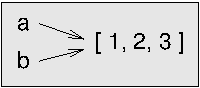
\includegraphics[scale=0.8]{../source/figs/list3.pdf}}
\caption{State diagram.}
\label{fig.list3}
\end{figure}

The association of a variable with an object is called a {\bf
reference}.  In this example, there are two references to the same
object.

变量和对象之间的关联称为 {\em 引用} (reference) 。
在这个例子中,有两个对同一个对象的引用。

\index{reference}

An object with more than one reference has more
than one name, so we say that the object is {\bf aliased}.

如果一个对象有多于一个引用,那它也会有多个名称,
我们称这个对象是 {\em 有别名的} (aliased) 。

\index{mutability}

If the aliased object is mutable, changes made with one alias affect
the other:

如果一个有别名的对象是可变的,对其中一个别名 (alias) 的改变对影响到其它的别名:

\begin{lstlisting}
>>> b[0] = 42
>>> a
[42, 2, 3]
\end{lstlisting}

%
Although this behavior can be useful, it is error-prone.  In general,
it is safer to avoid aliasing when you are working with mutable
objects.

尽管这个行为很有用,但是容易导致出现错误。
通常,避免对于可变对象使用别名相对更安全。

\index{immutability}

For immutable objects like strings, aliasing is not as much of a
problem.  In this example:

对于像字符串这样的不可变对象,使用别名没有什么问题。例如:

\begin{lstlisting}
a = 'banana'
b = 'banana'
\end{lstlisting}

%
It almost never makes a difference whether {\tt a} and {\tt b} refer
to the same string or not.

\li{a} 和 \li{b} 是否指向同一个字符串基本上没有什么影响。


\section{List arguments  |  列表参数}
\label{list.arguments}
\index{list!as argument}  \index{argument}
\index{argument!list}  \index{reference}
\index{parameter}

When you pass a list to a function, the function gets a reference to
the list.  If the function modifies the list, the caller sees
the change.  For example, \verb"delete_head" removes the first element
from a list:

当你将一个列表作为参数传给一个函数,函数将得到这个列表的一个引用。如果函数对这个列表进行了修改,会在调用者中有所体现。 例如, ``delete\_head'' 删除列表的第一个元素:

\begin{lstlisting}
def delete_head(t):
    del t[0]
\end{lstlisting}

%
Here's how it is used:

这样使用这个函数:

\begin{lstlisting}
>>> letters = ['a', 'b', 'c']
>>> delete_head(letters)
>>> letters
['b', 'c']
\end{lstlisting}

%
The parameter {\tt t} and the variable {\tt letters} are
aliases for the same object.  The stack diagram looks like
Figure~\ref{fig.stack5}.

参数 \li{t} 和变量 \li{letters} 是同一个对象的别名。
其堆栈图如图~\ref{fig.stack5}所示。

\index{stack diagram}  \index{diagram!stack}

\begin{figure}
\centerline
{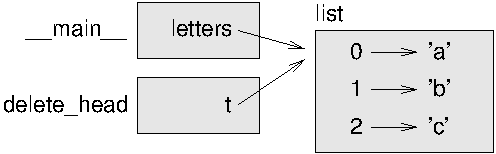
\includegraphics[scale=0.8]{../source/figs/stack5.pdf}}
\caption{Stack diagram.}
\label{fig.stack5}
\end{figure}

Since the list is shared by two frames, I drew
it between them.

由于列表被两个帧共享,我把它画在它们中间。

It is important to distinguish between operations that
modify lists and operations that create new lists.  For
example, the {\tt append} method modifies a list, but the
{\tt +} operator creates a new list:

需要注意的是修改列表操作和创建列表操作间的区别。
例如,\li{append} 方法是修改一个列表,而 \li{+} 运算符是创建一个新的列表:

\index{append method}  \index{method!append}
\index{list!concatenation}  \index{concatenation!list}

%
\begin{lstlisting}
>>> t1 = [1, 2]
>>> t2 = t1.append(3)
>>> t1
[1, 2, 3]
>>> t2
None
\end{lstlisting}

%
{\tt append} modifies the list and returns {\tt None}.

\li{append} 修改列表并返回 \li{None}。

%
\begin{lstlisting}
>>> t3 = t1 + [4]
>>> t1
[1, 2, 3]
>>> t3
[1, 2, 3, 4]
>>> t1
\end{lstlisting}

%
The {\tt +} operator creates a new list and leaves the
original list unchanged.

运算符 \li{+} 创建了一个新列表,而不改变原始的列表。

This difference is important when you write functions that
are supposed to modify lists.  For example, this function
{\em does not} delete the head of a list:

如果你要编写一个修改列表的函数,这一点就很重要。
例如,这个函数 {\em 不会} 删除列表的第一个元素:

%
\begin{lstlisting}
def bad_delete_head(t):
    t = t[1:]              # WRONG!
\end{lstlisting}

%
The slice operator creates a new list and the assignment
makes {\tt t} refer to it, but that doesn't affect the caller.

切片运算符创建了一个新列表,然后这个表达式让 \li{t} 指向了它,
但是并不会影响原来被调用的列表。

\index{slice operator}  \index{operator!slice}

%
\begin{lstlisting}
>>> t4 = [1, 2, 3]
>>> bad_delete_head(t4)
>>> t4
[1, 2, 3]
\end{lstlisting}

%
At the beginning of \verb"bad_delete_head", {\tt t} and {\tt t4}
refer to the same list.  At the end, {\tt t} refers to a new list,
but {\tt t4} still refers to the original, unmodified list.

在 \li{bad_delete_head} 的开始处,\li{t} 和 \li{t4} 指向同一个列表。在结束时,\li{t} 指向一个新列表,但是 \li{t4} 仍然指向原来的、没有被改动的列表。

An alternative is to write a function that creates and
returns a new list.  For example, {\tt tail} returns all but the first
element of a list:

一个替代的写法是,写一个创建并返回一个新列表的函数。
例如,\li{tail} 返回列表中除了第一个之外的所有元素:

\begin{lstlisting}
def tail(t):
    return t[1:]
\end{lstlisting}

%
This function leaves the original list unmodified.
Here's how it is used:

这个函数不会修改原来的列表。下面是函数的使用方法:

\begin{lstlisting}
>>> letters = ['a', 'b', 'c']
>>> rest = tail(letters)
>>> rest
['b', 'c']
\end{lstlisting}


\section{Debugging  |  调试}
\index{debugging}

Careless use of lists (and other mutable objects)
can lead to long hours of debugging.  Here are some common
pitfalls and ways to avoid them:

粗心地使用列表(以及其他可变对象)会导致长时间的调试。
下面列举一些常见的陷阱以及避免它们的方法:

\begin{enumerate}

\item Most list methods modify the argument and
  return {\tt None}.  This is the opposite of the string methods,
  which return a new string and leave the original alone.

If you are used to writing string code like this:

\begin{lstlisting}
word = word.strip()
\end{lstlisting}

It is tempting to write list code like this:

\begin{lstlisting}
t = t.sort()           # WRONG!
\end{lstlisting}
\index{sort method}
\index{method!sort}

Because {\tt sort} returns {\tt None}, the
next operation you perform with {\tt t} is likely to fail.

Before using list methods and operators, you should read the
documentation carefully and then test them in interactive mode.

\item Pick an idiom and stick with it.

Part of the problem with lists is that there are too many
ways to do things.  For example, to remove an element from
a list, you can use {\tt pop}, {\tt remove}, {\tt del},
or even a slice assignment.

To add an element, you can use the {\tt append} method or
the {\tt +} operator.  Assuming that {\tt t} is a list and
{\tt x} is a list element, these are correct:

\begin{lstlisting}
t.append(x)
t = t + [x]
t += [x]
\end{lstlisting}

And these are wrong:

\begin{lstlisting}
t.append([x])          # WRONG!
t = t.append(x)        # WRONG!
t + [x]                # WRONG!
t = t + x              # WRONG!
\end{lstlisting}

Try out each of these examples in interactive mode to make sure
you understand what they do.  Notice that only the last
one causes a runtime error; the other three are legal, but they
do the wrong thing.


\item Make copies to avoid aliasing.
\index{aliasing!copying to avoid}
\index{copy!to avoid aliasing}

If you want to use a method like {\tt sort} that modifies
the argument, but you need to keep the original list as
well, you can make a copy.

\begin{lstlisting}
>>> t = [3, 1, 2]
>>> t2 = t[:]
>>> t2.sort()
>>> t
[3, 1, 2]
>>> t2
[1, 2, 3]
\end{lstlisting}

In this example you could also use the built-in function {\tt sorted},
which returns a new, sorted list and leaves the original alone.

\begin{lstlisting}
>>> t2 = sorted(t)
>>> t
[3, 1, 2]
>>> t2
[1, 2, 3]
\end{lstlisting}

\end{enumerate}


\begin{enumerate}

\item 大多数的列表方法会对参数进行修改,然后返回 \li{None} 。这和字符串方法相反,后者保留原始的字符串并返回一个新的字符串。

如果你习惯这样写字符串代码:

\begin{lstlisting}
word = word.strip()
\end{lstlisting}

那么你很可能会写出下面的列表代码:

\begin{lstlisting}
t = t.sort()           # WRONG!
\end{lstlisting}
\index{sort method}
\index{method!sort}

因为 \li{sort} 返回 \li{None} ,所以你的下一个对 \li{t} 执行的操作很可能会失败。

在使用 \li{list} 方法和操作符之前,你应该仔细阅读文档,然后在交互模式下测试。

\item 选择一种写法,坚持下去。

列表的一个问题就是有太多方法可以做同样的事情。  例如,要删除列表中的一个元素,你可以使用 \li{pop} 、 \li{remove} 、 \li{del} 甚至是切片赋值。

 要添加一个元素,你可以使用 \li{append} 方法或者 \li{+} 运算符。 假设 \li{t} 是一个列表,\li{x} 是一个列表元素,以下这些写法都是正确的:

\begin{lstlisting}
t.append(x)
t = t + [x]
t += [x]
\end{lstlisting}

而这些是错误的:

\begin{lstlisting}
t.append([x])          # WRONG!
t = t.append(x)        # WRONG!
t + [x]                # WRONG!
t = t + x              # WRONG!
\end{lstlisting}

在交互模式下尝试每一个例子,保证你明白它们做了什么。  注意只有最后一个会导致运行时错误;其他的都是合乎规范的的,但结果却是错的。


\item 通过创建拷贝来避免别名.
\index{aliasing!copying to avoid}  \index{copy!to avoid aliasing}

如果你要使用类似 \li{sort} 这样的方法来修改参数,
   但同时有要保留原列表,你可以创建一个拷贝。


\begin{lstlisting}
>>> t = [3, 1, 2]
>>> t2 = t[:]
>>> t2.sort()
>>> t
[3, 1, 2]
>>> t2
[1, 2, 3]
\end{lstlisting}

在这个例子中,你还可以使用内置函数 \li{sorted}, 它将返回一个新的已排序的列表,原列表将保持不变。

\begin{lstlisting}
>>> t2 = sorted(t)
>>> t
[3, 1, 2]
>>> t2
[1, 2, 3]
\end{lstlisting}

\end{enumerate}


\section{Glossary  |  术语表}

\begin{description}

\item[list:] A sequence of values.
\index{list}

\item[列表(list):] 多个值组成的序列。
\index{list}

\item[element:] One of the values in a list (or other sequence),
also called items.
\index{element}

\item[元素(element):] 列表(或序列)中的一个值,也称为项。
\index{element}

\item[nested list:] A list that is an element of another list.
\index{nested list}

\item[嵌套列表(nested list):] 作为另一个列表的元素的列表。
\index{nested list}

\item[accumulator:] A variable used in a loop to add up or
accumulate a result.
\index{accumulator}

\item[累加器(accumulator):] 循环中用于相加或累积出一个结果的变量。
\index{accumulator}

\item[augmented assignment:] A statement that updates the value
of a variable using an operator like \verb"+=".
\index{assignment!augmented}  \index{augmented assignment}
\index{traversal}

\item[增量赋值语句(augmented assignment):] 一个使用类似 \li{+=} 操作符来更新一个变量的值的语句。
\index{assignment!augmented}  \index{augmented assignment}
\index{traversal}

\item[reduce:] A processing pattern that traverses a sequence
and accumulates the elements into a single result.
\index{reduce pattern}  \index{pattern!reduce}

\item[归并(reduce):] 遍历序列,将所有元素求和为一个值的处理模式。
\index{reduce pattern}  \index{pattern!reduce}

\item[map:] A processing pattern that traverses a sequence and
performs an operation on each element.
\index{map pattern}  \index{pattern!map}

\item[映射(map):] 遍历序列,对每个元素执行操作的处理模式。
\index{map pattern}  \index{pattern!map}

\item[filter:] A processing pattern that traverses a list and
selects the elements that satisfy some criterion.
\index{filter pattern}  \index{pattern!filter}

\item[筛选(filter):] 遍历序列,选出满足一定标准的元素的处理模式。
\index{filter pattern}  \index{pattern!filter}

\item[object:] Something a variable can refer to.  An object
has a type and a value.
\index{object}

\item[对象(object)] 变量可以指向的东西。一个对象有数据类型和值。
\index{object}

\item[equivalent:] Having the same value.
\index{equivalent}

\item[相等(equivalent):] 有相同的值。
\index{equivalent}

\item[identical:] Being the same object (which implies equivalence).
\index{identical}

\item[相同(identical):] 是同一个对象(隐含着相等)。
\index{identical}

\item[reference:] The association between a variable and its value.
\index{reference}

\item[引用(reference):] 一个变量和它的值之间的关联。
\index{reference}

\item[aliasing:] A circumstance where two or more variables refer to the same
object.
\index{aliasing}

\item[别名使用:] 两个或者两个以上变量指向同一个对象的情况。
\index{aliasing}

\item[delimiter:] A character or string used to indicate where a
string should be split.
\index{delimiter}

\item[分隔符(delimiter):] 一个用于指示字符串分割位置的字符或者字符串。
\index{delimiter}

\end{description}


\section{Exercises  |  练习}

You can download solutions to these exercises from
\url{http://thinkpython2.com/code/list_exercises.py}.

你可以从 \href{http://thinkpython2.com/code/list_exercises.py}{此处} 下载这些练习的答案。

\begin{exercise}

Write a function called \verb"nested_sum" that takes a list of lists
of integers and adds up the elements from all of the nested lists.
For example:

编写一个叫做 \li{nested_sum} 的函数, 接受一个由一些整数列表构成的列表作为参数, 并将所有嵌套列表中的元素相加。 例如:

\begin{lstlisting}
>>> t = [[1, 2], [3], [4, 5, 6]]
>>> nested_sum(t)
21
\end{lstlisting}

\end{exercise}

\begin{exercise}
\label{cumulative}
\index{cumulative sum}

Write a function called {\tt cumsum} that takes a list of numbers and
returns the cumulative sum; that is, a new list where the $i$th
element is the sum of the first $i+1$ elements from the original list.
For example:

编写一个叫做 \li{cumsum} 的函数,接受一个由数值组成的列表,并返回累加和;
即一个新列表,其中第 $i+1$ 个元素是原列表中前 $i$ 个元素的和。
例如:

\begin{lstlisting}
>>> t = [1, 2, 3]
>>> cumsum(t)
[1, 3, 6]
\end{lstlisting}

\end{exercise}

\begin{exercise}

Write a function called \verb"middle" that takes a list and
returns a new list that contains all but the first and last
elements.  For example:

编写一个叫做 \li{middle} 的函数,接受一个列表作为参数,并返回一个除了第一个和最后一个元素的列表。
例如:


\begin{lstlisting}
>>> t = [1, 2, 3, 4]
>>> middle(t)
[2, 3]
\end{lstlisting}

\end{exercise}

\begin{exercise}

Write a function called \verb"chop" that takes a list, modifies it
by removing the first and last elements, and returns {\tt None}.
For example:

编写一个叫做 \li{chop} 的函数,接受一个列表作为参数,移除第一个和最后一个元素,并返回 \li{None}。
例如:

\begin{lstlisting}
>>> t = [1, 2, 3, 4]
>>> chop(t)
>>> t
[2, 3]
\end{lstlisting}

\end{exercise}


\begin{exercise}
Write a function called \verb"is_sorted" that takes a list as a
parameter and returns {\tt True} if the list is sorted in ascending
order and {\tt False} otherwise.  For example:

编写一个叫做 \li{is_sorted} 的函数,接受一个列表作为参数,
如果列表是递增排列的则返回 \li{True} ,否则返回 \li{False}。
例如:

\begin{lstlisting}
>>> is_sorted([1, 2, 2])
True
>>> is_sorted(['b', 'a'])
False
\end{lstlisting}

\end{exercise}


\begin{exercise}
\label{anagram}
\index{anagram}

Two words are anagrams if you can rearrange the letters from one
to spell the other.  Write a function called \verb"is_anagram"
that takes two strings and returns {\tt True} if they are anagrams.


如果可以通过重排一个单词中字母的顺序,得到另外一个单词,那么称这两个单词是变位词。
编写一个叫做 \li{is_anagram} 的函数,接受两个字符串作为参数,
如果它们是变位词则返回 \li{True} 。
\end{exercise}



\begin{exercise}
\label{duplicate}
\index{duplicate}  \index{uniqueness}

Write a function called \verb"has_duplicates" that takes
a list and returns {\tt True} if there is any element that
appears more than once.  It should not modify the original
list.

编写一个叫做 \li{has_duplicates} 的函数,接受一个列表作为参数,
如果一个元素在列表中出现了不止一次,则返回 \li{True} 。
这个函数不能改变原列表。

\end{exercise}


\begin{exercise}

This exercise pertains to the so-called Birthday Paradox, which you
can read about at \url{http://en.wikipedia.org/wiki/Birthday_paradox}.
\index{birthday paradox}

这个习题与所谓的生日悖论有关。
你可以在 \href{http://en.wikipedia.org/wiki/Birthday_paradox}{此处}了解更多相关的内容。

If there are 23 students in your class, what are the chances
that two of you have the same birthday?  You can estimate this
probability by generating random samples of 23 birthdays
and checking for matches.  Hint: you can generate random birthdays
with the {\tt randint} function in the {\tt random} module.

如果你的班级上有 23 个学生, 2 个学生生日相同的概率是多少?
你可以通过随机产生 23 个生日,并检查匹配来估算概率。
提示:你可以使用 \li{random} 模块中的 \li{randint} 函
数来生成随机生日。

\index{random module}  \index{module!random}
\index{randint function}  \index{function!randint}

You can download my
solution from \url{http://thinkpython2.com/code/birthday.py}.

你可以参考 \href{http://thinkpython2.com/code/birthday.py}{我的答案}。

\end{exercise}



\begin{exercise}
\index{append method}  \index{method append}
\index{list!concatenation}  \index{concatenation!list}

Write a function that reads the file {\tt words.txt} and builds
a list with one element per word.  Write two versions of
this function, one using the {\tt append} method and the
other using the idiom {\tt t = t + [x]}.  Which one takes
longer to run?  Why?

编写一个函数,读取文件 \li{words.txt},建立一个列表,其中每个单词为一个元素。
编写两个版本,一个使用 \li{append} 方法,另一个使用 \li{t = t + [x]}。
那个版本运行得慢?为什么?

Solution: \url{http://thinkpython2.com/code/wordlist.py}.

\href{http://thinkpython2.com/code/wordlist.py}{参考答案}

\index{time module}  \index{module!time}

\end{exercise}


\begin{exercise}
\label{wordlist1}
\label{bisection}
\index{membership!bisection search}  \index{bisection search}
\index{search, bisection}  \index{membership!binary search}
\index{binary search}  \index{search, binary}

To check whether a word is in the word list, you could use
the {\tt in} operator, but it would be slow because it searches
through the words in order.

使用 \li{in} 运算符可以检查一个单词是否在单词表中, 但这很慢, 因为它是按顺序查找单词。

Because the words are in alphabetical order, we can speed things up
with a bisection search (also known as binary search), which is
similar to what you do when you look a word up in the dictionary.  You
start in the middle and check to see whether the word you are looking
for comes before the word in the middle of the list.  If so, you
search the first half of the list the same way.  Otherwise you search
the second half.

由于单词是按照字母顺序排序的,我们可以使用两分法(也称二进制搜索)来加快速度,
类似你在字典中查找单词的方法。 你从中间开始,如果你要找的单词在中间的单词之前,你查找前半部分,否则你查找后半部分。

Either way, you cut the remaining search space in half.  If the
word list has 113,809 words, it will take about 17 steps to
find the word or conclude that it's not there.

不管怎样,你都会将搜索范围减小一半。
如果单词表有 113,809 个单词,你只需要 17步就可以找到这个单词,或着得出单词不存在的结论。

Write a function called \verb"in_bisect" that takes a sorted list
and a target value and returns the index of the value
in the list if it's there, or {\tt None} if it's not.

编写一个叫做 \li{in_bisect} 的函数,接受一个已排序的列表和一个目标值作为参数,
返回该值在列表中的位置,如果不存在则返回 \li{None} 。

\index{bisect module}  \index{module!bisect}

Or you could read the documentation of the {\tt bisect} module
and use that!  Solution: \url{http://thinkpython2.com/code/inlist.py}.

或者你可以阅读 \li{bisect} 模块的文档并使用它!

\href{http://thinkpython2.com/code/inlist.py}{参考答案}

\end{exercise}

\begin{exercise}
\index{reverse word pair}

Two words are a ``reverse pair'' if each is the reverse of the
other.  Write a program that finds all the reverse pairs in the
word list.  Solution: \url{http://thinkpython2.com/code/reverse_pair.py}.

两个单词中如果一个是另一个的反转,则二者被称为是``反转词对''。
编写一个函数,找出单词表中所有的反转词对。

\href{http://thinkpython2.com/code/reverse_pair.py}{参考答案}

\end{exercise}

\begin{exercise}
\index{interlocking words}

Two words ``interlock'' if taking alternating letters from each forms
a new word.  For example, ``shoe'' and ``cold''
interlock to form ``schooled''.
Solution: \url{http://thinkpython2.com/code/interlock.py}.
Credit: This exercise is inspired by an example at \url{http://puzzlers.org}.

如果交替的从两个单词中取出字符将组成一个新的单词,这两个单词被称为是``连锁词''。
例如,``shoe'' 和 ``cold'' 连锁后成为 ``schooled''。

\begin{enumerate}

\item Write a program that finds all pairs of words that interlock.
  Hint: don't enumerate all pairs!

\item 编写一个程序,找出单词表中所有的连锁词。提示:不要枚举所有的单词对。

\item Can you find any words that are three-way interlocked; that is,
  every third letter forms a word, starting from the first, second or
  third?

\item 你能够找到三重连锁的单词吗?即每个字母依次从3个单词得到。

\end{enumerate}
\end{exercise}